\documentclass[a4paper]{article}
\usepackage[utf8x]{inputenc}
\usepackage[T1,T2A]{fontenc}
\usepackage[russian]{babel}
\usepackage{hyperref}
\usepackage{indentfirst} % включить отступ у первого абзаца
\usepackage{listings}
\lstset{inputpath=../listings}
\usepackage{color}
\usepackage{here} 
\usepackage{graphicx}
\graphicspath{{pics/}}

\usepackage{caption}
\renewcommand{\lstlistingname}{Листинг}

\usepackage{listings}
\lstdefinestyle{base_listing}{ %
extendedchars=\true,
basicstyle=\footnotesize,       % the size of the fonts that are used for the code
numbers=left,                   % where to put the line-numbers
numberstyle=\footnotesize,      % the size of the fonts that are used for the line-numbers
stepnumber=1,                   % the step between two line-numbers. If it is 1 each line will be numbered
numbersep=5pt,                  % how far the line-numbers are from the code
backgroundcolor=\color{white},  % choose the background color. You must add \usepackage{color}
showspaces=false,               % show spaces adding particular underscores
showstringspaces=false,         % underline spaces within strings
showtabs=false,                 % show tabs within strings adding particular underscores
frame=single,           % adds a frame around the code
tabsize=2,          % sets default tabsize to 2 spaces
captionpos=b,           % sets the caption-position to bottom
breaklines=true,        % sets automatic line breaking
breakatwhitespace=false,    % sets if automatic breaks should only happen at whitespace
escapeinside={\%*}{*)},          % if you want to add a comment within your code
postbreak=\raisebox{0ex}[0ex][0ex]{\ensuremath{\color{red}\hookrightarrow\space}},
keepspaces = true
}

\lstdefinestyle{crs_bash}{
  style    = {base_listing},
  language = {bash}
}

\lstdefinestyle{crs_cpp}{
  style    = {base_listing},
  language = {C++}
}

\usepackage[left=2.5cm, top=2cm, right=2cm, bottom=2cm, nohead]{geometry}

\begin{document}
\begin{titlepage} % начало титульной страницы

\begin{center} % включить выравнивание по центру

\large Санкт-Петербургский Политехнический Университет Петра Великого\\
\large Институт компьютерных наук и технологий \\
\large Кафедра компьютерных систем и программных технологий\\[6cm]
% название института, затем отступ 4,5см

\huge Операционные системы и среды\\[0.5cm]
\large Отчет по лабораторной работе №8\\[0.1cm]
\large Средства синхронизации потоков и процессов в ОС Linux и
их применение\\[5cm]
\end{center}

\begin{flushright}
\begin{minipage}{0.5\textwidth}
\begin{flushright}
\textbf{Работу выполнил:}

Петров Владислав

{Группа:} 43501/4\\


\textbf{Преподаватель:} 

Душутина Елена Владимировна
\end{flushright}
\end{minipage} % конец врезки
\end{flushright} % конец выравнивания по левому краю

\vfill % заполнить всё доступное ниже пространство

\begin{center}

\large Санкт-Петербург\\
\large \the\year % вывести дату

\end{center} % закончить выравнивание по центру

\thispagestyle{empty} % не нумеровать страницу
\end{titlepage} % конец титульной страницы

\vfill % заполнить всё доступное ниже пространство


\section{Цель работы}
	Изучение средств синхронизации потоков и процессов в ОС семейства Linux и
их применение.
	
\section{Программа работы}
\begin{enumerate}
\item Привести собственные результаты выполнения предложенных программ и  их анализ. 
\item Модифицировать предложенное решение таким образом, чтобы «читатели» не имели  доступа к памяти по записи. 
\item Предложить  более  рациональное  решение  задачи  «читатели-писатель»,  используя другие  средства  синхронизации  или  их  сочетание.  Объяснить  и  подтвердить экспериментально улучшение характеристик взаимодействия.
\item Разработать  клиент-серверное  приложение  для  полной задачи  «читатели-писатели»  с собственной системой ограничений на доступ каждого «читателя» к информации.
\item  Разработать  программу «читатели-писатели»  для  сетевого  функционирования.  Для этого выбрать подходящие средства IPC и  синхронизации.
\item Предложить  программное  решение  задачи  «производители-потребители».  Разница  с предыдущей задачей – возможность модификации считываемых данных.
\item Решить   задачу   «обедающие   философы», обосновать выбранные средства синхронизации.
\end{enumerate}

\section{Ход работы}
	Лабораторная выполняется на физической машине со следующими характеристиками:
	\lstinputlisting[style=crs_bash]{../listings/uname}

\subsection{Создание двух потоков: потока – производителя и потока – потребителя}
	\textbf{Задание.} Создание двух потоков: потока – производителя и потока – потребителя.
Потоки разделяют целочисленный массив, в который заносятся производимые и извлекаются потребляемые данные. Для наглядности и контроля за происходящим в буфер помещается наращиваемое значение, однозначно идентифицирующее производителя и номер его очередной посылки.
Код должен удовлетворять трем требованиям:\begin{itemize}
\item потребитель не должен пытаться извлечь значение из буфера, если буфер пуст;
\item производитель не должен пытаться поместить значение в буфер, если буфер полон;
\item состояние буфера должно описываться общими переменными (индексами, счетчиками, указателями связанных списков и т.д.).
\end{itemize}
Задание необходимо выполнить различными способами, применив следующие средства синхронизации доступа к разделяемому ресурсу:
\begin{itemize}
\item Мьютексы;
\item Семафоры;
\end{itemize}
Программы должны предоставлять возможность завершения по таймеру либо по команде оператора.
\textbf{Решение.}
Структурируем программу так, чтобы по изменению одного константного значения можно было запускать программу для разных средств синхронизации. Для этого будем использовать прекомпиляцию
	\begin{lstlisting}[style=crs_cpp]
#define TYPE_OF_SYNCHRONISE 1
enum //описание значений
{
	MUTEX = 0,
	SEM = 1,
	CRS = 2,
	EVENT =  3,
	COND =4
};
	\end{lstlisting}
	В нашем случае используются только два первых константных значения: 0 и 1
Данные параметры загружаются в структуру вида:
	\begin{lstlisting}[style=crs_cpp]
struct Configuration 
{ 
int numOfReaders; //число потоков-читателей 
int numOfWriters; //число потоков-писателей 
int sizeOfQueue;  //размер очереди 
int readersDelay; //задержка на работу читателей (в миллисек) 
int writersDelay; //задержка на работу писателей (в миллисек) 
int ttl; //"время жизни" 
};
	\end{lstlisting}
Вся конфигурационная информация загружается из файла, имеющего следующий вид:

	\begin{lstlisting}[style=crs_cpp]
NumOfReaders= 10 
ReadersDelay= 100 
NumOfWriters= 10 
WritersDelay= 200 
SizeOfQueue= 10 
ttl= 3
	\end{lstlisting}
Очередь определяется в виде структуры:
	\begin{lstlisting}[style=crs_cpp]
struct FIFOQueue //FIFO очередь 
{ 
char **data; 	//массив сообщений 
int writeindex; //индекс записи 
int getindex; 	//индекс чтения 
int size; 		//размер очереди 
short full; 	//очередь заполнена 
};
	\end{lstlisting}

	Результат выполнения программы приведен на рисунке \ref{img:alg_main_thread}.
	\begin{figure}[h!]
		\center{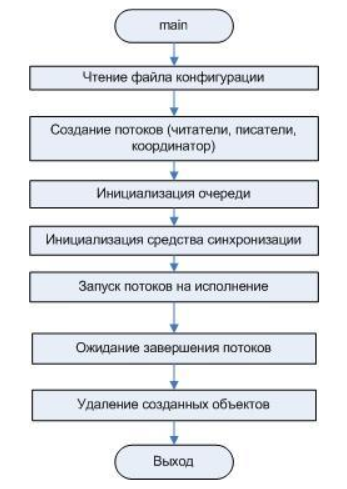
\includegraphics[scale=0.8]{alg_main_thread}}
		\caption{Схема алгоритма работы главного потока}
		\label{img:alg_main_thread}
	\end{figure}

	Исходный код функции главного потока:
	\lstinputlisting[style=crs_cpp]{../listings/m_thread.c}
	Для структурирования кода использованы вспомогательные функции.
Функция SetConfig – производит чтение конфигурационного файла и заполнение структуры config. Функция CreateAllThreads – создает все потоки (читатели, писатели, координатор).\\

Исходный код вспомогательных функций:
	\lstinputlisting[style=crs_cpp]{../listings/assist.c}
	
	Схема алгоритма работы потока-координатора представлена на рис \ref{img:thr_coord}.
	\begin{figure}[h!]
		\center{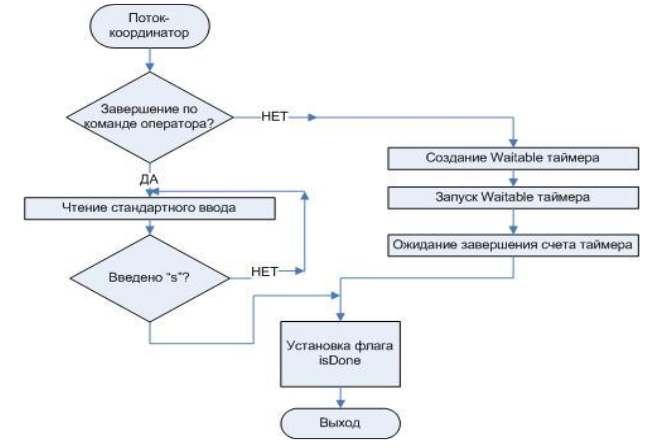
\includegraphics[scale=0.8]{thr_coord}}
		\caption{Схема алгоритма работы потока-координатора}
		\label{img:thr_coord}
	\end{figure}
	
	Исходный код функции потока-координатора:
	\lstinputlisting[style=crs_cpp]{../listings/coord.c}

	Схема алгоритма работы потока-читателя представлена на рис \ref{img:thr_reader}.
	\begin{figure}[h!]
		\center{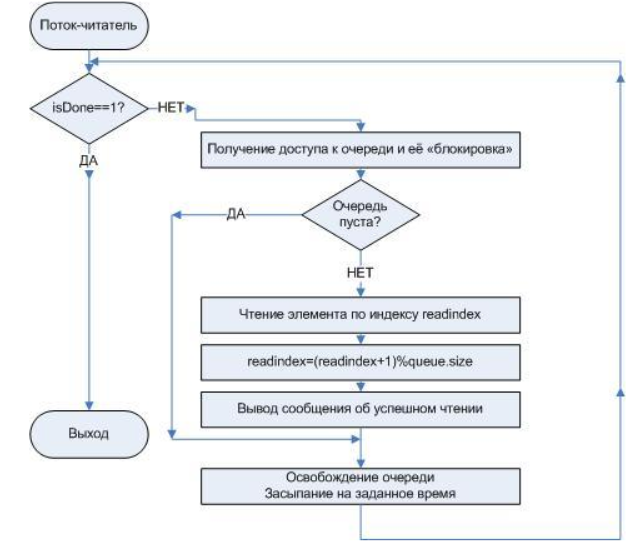
\includegraphics[scale=0.8]{thr_reader}}
		\caption{Схема алгоритма работы потока-читателя}
		\label{img:thr_reader}
	\end{figure}
	Исходный код потока-читателя:
	\lstinputlisting[style=crs_bash]{../listings/reader.c}
	Программа готова к запуску, необходимо лишь изменять константное значение.
	В дальнейшем используется следующая конфигурация:
	\begin{lstlisting}[style=crs_cpp]
NumOfReaders= 3 
ReadersDelay= 1 
NumOfWriters= 4 
WritersDelay= 1 
SizeOfQueue= 5 
ttl= 3
	\end{lstlisting}
	
\subsection{Использование мьютексов в качестве средства синхронизации}
Запускаем программу со значением константы TYPE\_OF\_SYNCHRONISE = 0
В данном случае мы используем мьютекс из библиотеки pthread.h. Такой мьютекс не является обьектом ядра, поэтому может синхронизировать только потоки, а не процессы.\\

Результат выполнения программы:
	\lstinputlisting[style=crs_bash]{../listings/mutex_log}
	12 записей и 7 считываний. Т.к. данный мьютекс не является объектом ядра, то он должен быть похож на критические секции ОС Windows. Предположительно он должен работать быстрее семафоров.

\subsection{Использование семафоров в качестве средства синхронизации}
Запустим программу с константой TYPE\_OF\_SYNCHRONISE = 1
Результаты выполнения:
	\lstinputlisting[style=crs_bash]{../listings/sem_log}
12 записей и 8 считываний. Получилось немного быстрее чем с мьютексем, однако проводимый тест включает в себя мало функций чтения/записи. В других условиях результаты могут поменяться. В данном тесте семафор использован так же как и мьютекс, в то время как семафор может быть «многоуровневым», поэтому в данном примере потенциал семафора использован не полностью

\subsection{Решение задачи «читатели-писатели» для потоков разных процессов с синхронизацией объектами}
В данной программе главный поток и поток-писатель будут принадлежать одному процессу, потоки-читатели – разным. Главный процесс создает процессы-читатели и 2 потока: писатель и планировщик. Для наглядности каждый процесс-читатель связан со своей консолью.\\

Писатель захватывает первый сумафор, пишет сообщение, записывает счетчик прочитавших в начало файла, освобождает семафор для чтения читателями.
	\lstinputlisting[style=crs_cpp]{../listings/sem_writer.c}
	Читатель ожидает освобождения семафора для чтения, читает, изменяет счетчик прочитавших, ожидает пока счетчик не станет равным 0(все прочитали), освобождает первый семафор на запись. 
Процесс читателя:
	\lstinputlisting[style=crs_cpp]{../listings/sem_reader.c}
Результат выполнения:
	\lstinputlisting[style=crs_bash]{../listings/sem_rw}
	Потоки читатели читают повторно, чего быть не должно.
	
\subsection{Обедающие философы}
Классическая формулировка задачи
Рассмотрим формулировку задачи об обедающих философах в терминологии, предложенной Э. Дейкстрой. За круглым столом расставлены пять стульев, на каждом из которых сидит философ (Ф1-Ф5) 
	\begin{figure}[h!]
		\center{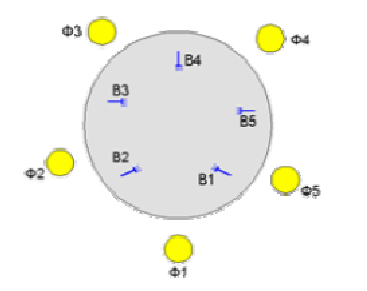
\includegraphics[scale=0.8]{phi}}
		\caption{Схема задачи о философах}
		\label{img:phi}
	\end{figure}
В центре стола размещено блюдо с макаронами. На столе лежат пять вилок (B1-B5), каждая из которых находится между двумя соседними тарелками. Каждый философ может находиться в двух состояниях: размышлять или есть макароны. Для того, чтобы начать есть, философу необходимы две вилки: одна в правой руке, а другая в левой. Закончив еду, философ кладет вилки на место и начинает размышлять до тех пор, пока снова не проголодается.
В этой задаче имеются две опасные ситуации: «заговор соседей» и «голодная смерть». 
«Заговор соседей» имеет место, когда соседи слева и справа от философа строят козни. Заговорщики поочередно забирают вилки то слева, то справа от «жертвы». Такие согласованные действия злоумышленников приводят жертву к вынужденному голоданию, так как он никогда не может воспользоваться обеими вилками.
«Голодная смерть» возникает, когда философы одновременно проголодаются и одновременно попытаются взять, например, свою левую вилку. При этом возникает тупиковая ситуация, так как никто из них не может начать есть, не имея второй вилки.\\

\textbf{Формулировка решаемой задачи}
Для устранения неоднозначности поведения философа была предложена следующая
модель его поведения:
размышляет -> берет левую вилку -> берет правую вилку -> ест -> кладет правую вилку -> кладет левую вилку -> размышляет.
При такой модели поведения философа проблема «заговора соседей» отпадает, так как каждый философ рано или поздно насытится, а значит, освободит вилку. Остается решить проблему «голодной смерти». Для этого в задачу введен еще один персонаж — «Официант». Он должен следить за тем, чтобы в столовой не находилось более четырех философов одновременно.

\textbf{Алгоритм работы}
Опираясь на формулировку поставленной задачи, соотнесем каждой вилке мьютекс, для того чтобы только один философ мог единовременно держать её в руках. Вместо официанта введем семафор размерностью N-1, где N – число философов.
Таким образом, алгоритм каждого философа сводится к следующим действиям:
Размышляет->ожидает разрешения официанта -> пытается взять вилку справа -> пытается взять вилку слева -> кушает -> кладет правую вилку -> кладет левую вилку -> размышляет.


Реализация
В программе убрано создание потоков читателей, а потоки писатели становятся философами.
Функция main и обьявление переменных:
	\lstinputlisting[style=crs_cpp]{../listings/phi_sam7.c}
Функция-поток, отвечающая за действия одного философа
	\lstinputlisting[style=crs_cpp]{../listings/phi_foo.c}
Результаты работы:
	\lstinputlisting[style=crs_bash]{../listings/phi_log}
	

Анализируя результат выполнения программы видно, что
\begin{enumerate}
\item Все философы употребляют пищу в равной мере.
\item Нет голодающих философов
\item Отсутствуют некорректные ситуации, когда одна вилка захвачена двумя философами, наоборот видно, как один из философов ждет освобождения вилки другим.
\item Не возникает ситуации взаимной блокировки, когда все философы держат по одной вилке и бесконечно ожидают другой.
\end{enumerate}
Используя один многоуровневый семафор и мьютексы(одноуровненвый семафор), нам удалось решить задачу обедающих философов. Существуют и другие пути реализации данной задачи. Также в созданной программе не происходит оптимизации, доступа к пище, но это и не являлось условием задачи.

\section{Вывод}
В данной работе мы изучили средства синхронизации потоков и процессов операционной системы Linux. Мы познакомились со средствами ядра, такими как мьютексы и семафоры. С использованием семафоров была решена задача обедающих философов. Поставлены эксперименты с данными средствами синхронизации. Стоит заметить что в ОС Linux использование средств синхронизации в чем то более сложное, а в чем то проще. Например, в ОС Windows нам необходимо задавать параметры безопастности чтобы другие процессы смогли пользоваться, к примеру, семафором. С другой стороны в Linux используется файл-ключ, который сначала необходимо инициализировать. 

\section{Список литературы}
\begin{itemize}
\item Душутина Е.В.  Межпроцессные взаимодействия в операционных системах – СПб, 2014 г, 136 с.
\item Душутина Е.В.  Практические вопросы оазработки системных приложений – СПб, 2015 г, 165 с.
\item Таненбаум Э., Бос Х. Современные операционные системы. 4-е изд. – СПб.: Питер, 2015 – 1120 с.
\item С.В.Пакб А.А.Шалыто. Задача об обедающих философах. URL: http://is.ifmo.ru/download/phil.pdf (Просмотрен 29.03.2016)
\end{itemize}
	
	

\end{document}

